
\section{动机与总体规划}

设 $X$ 是一个「\trSmooth」的 $k$-\trVariety。我们想定义\trTangentBundle。我们将会看到，做这件事的正确方式可以轻而易举地适用于广泛得多的情形。

\begin{itemize}[leftmargin=2.6em,itemsep=2pt,topsep=3pt]
\item 我们将会看到，对\trScheme{}而言，\trCotangentSheaf（cotangent sheaf）比\trTangentBundle{}或\trTangentSheaf{}更为「自然」。这类似于「\trZariski{}\trCotangentSpace{}比\trTangentSpace{}更自然」这一事实（也就是说，若 $A$ 是一个\trRing{}而 $\mathfrak{m}$ 是一个\trMaximalIdeal，则 $\mathfrak{m}/\mathfrak{m}^2$ 比 $(\mathfrak{m}/\mathfrak{m}^2)^{\vee}$ 「更自然」），自 \S13.1 以来我们已反复讨论过这一点。在两种情形下，缘由都在于：我们是通过「空间」上的函数（层）来理解「空间」的，而这与你心目中关于空间的几何图像在某种意义上互为对偶。所以我们将先定义\trCotangentSheaf。（余）\trTangentSpace{}的元素将称为\textbf{（余）\trTangentVector}。
\item 我们本科阶段的直觉会继续奏效——我们可以用\trJacobianMatrix{}进行计算，在本科式计算适用的那些情形里答案也相同，而且我们甚至还有避开 $\delta$ 与 $\epsilon$ 的额外优势。
\item 我们的构造会自动适用于一般的 $X$，哪怕 $X$ 不\trSmooth（甚至压根谈不上「好」，比如连\trFiniteType{}都不是）也照样适用。\trCotangentSheaf{}未必\trLocallyFree，但它仍将是一个\trQCSheaf。
\item 更妙的是，这一构造还会自然而然地以「相对」的方式奏效。对任意 $\pi\colon X\to Y$，我们将定义 $\Omega_\pi=\Omega_{X/Y}$，即 $X$ 上的一个\trQCSheaf——相对微分层（sheaf of relative differentials）。这个层在某一点处的\trFiber{}将是映射的纤维的诸\trCotangentVector。取 $Y=\Spec k$，便特化为此前的情形。其想法是：它把这个族的诸纤维的\trCotangentSheaf{}黏合在一起。图~\ref{fig:relative-tangent-space}便是映射 $X\to Y$ 在一点 $\mathrm{p}\in X$ 处的相对\trTangentSpace{}的草图——它就是纤维的切空间。（\trTangentSpace{}总比\trCotangentSpace{}容易画！）相对（余）\trTangentSpace{}的元素则称为\textbf{相对（余）\trTangentVector}。
\end{itemize}

\begin{figure}[htbp]
\centering
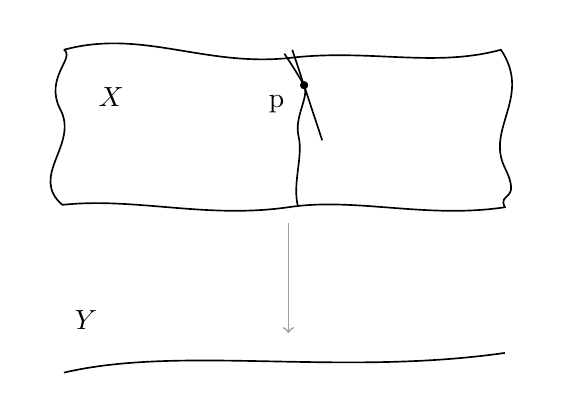
\begin{tikzpicture}[semithick]
  \draw (1.0,5.05)
    .. controls (2.0,5.32) and (2.8,4.82) .. (3.9,4.95)
    .. controls (4.9,5.06) and (5.7,4.82) .. (6.55,5.05)
    .. controls (6.95,4.45) and (6.35,4.05) .. (6.6,3.55)
    .. controls (6.82,3.10) and (6.50,3.25) .. (6.6,3.05)
    .. controls (5.6,2.90) and (4.7,3.18) .. (3.85,3.05)
    .. controls (2.8,2.90) and (1.9,3.18) .. (0.98,3.08)
    .. controls (0.55,3.45) and (1.20,3.85) .. (0.95,4.30)
    .. controls (0.75,4.70) and (1.15,4.95) .. (1.0,5.05);
  \draw (3.80,5.00) .. controls (3.90,4.85) and (3.98,4.72) .. (4.05,4.60)
        .. controls (4.12,4.45) and (3.92,4.20) .. (3.98,3.95)
        .. controls (4.04,3.70) and (3.90,3.35) .. (3.97,3.07);
  \draw (3.90,5.05) -- (4.28,3.90);
  \fill (4.05,4.60) circle (1.5pt);
  \draw[gray!75,->] (3.85,2.85) -- (3.85,1.45);
  \draw (1.0,0.95) .. controls (2.5,1.30) and (4.5,0.90) .. (6.6,1.20);
  \node at (1.60,4.45) {$X$};
  \node at (3.70,4.36) {$\mathrm{p}$};
  \node at (1.28,1.62) {$Y$};
\end{tikzpicture}
\caption{态射 $X\to Y$ 在一点 $\mathrm{p}$ 处的相对\trTangentSpace。（依原书手绘图重绘。）}
\label{fig:relative-tangent-space}
\end{figure}

于是，本章的中心概念便是：对概形的\trMorphism{} $\pi\colon X\to Y$ 而言的\trCotangentSheaf $\Omega_\pi=\Omega_{X/Y}$。在你心目中值得保有的一幅图景如下。若 $\pi\colon X\to Y$ 是\trManifold{}之间的一个\trSubmersion（一个在诸\trTangentSpace{}上诱导满射的映射），你或许会指望：诸纤维在各点 $\mathrm{p}\in X$ 处的\trTangentSpace{}能拼合起来，构成一个\trVectorBundle。这就是（$\pi$ 的）相对\trTangentBundle，而它的\trDual{}就是 $\Omega_{X/Y}$（见图~\ref{fig:relative-tangent-space}）。即使你并不以几何的方式思考问题，你也会发现这很有用。（算术方面的例子，参看\mbox{练习~21.2.H}。）
